\chapter{Results}
This chapter is dedicated to the results of model testing on users, as well as the impact of features and hyperparameter choices on its performance. 

\section{Model Performance on User Data}
This section focuses on the results of testing the collection of models that were found to have the best performance during validation. It aims to show the how this solution performs on the unseen test dataset as well as highlight the large differences between individual models within the collection of models.

\subsection{Methodology}
The results below were calculated as an average of each models performance on a sequence of characters equal to the length on which the model was trained.
This means that were tested with input of different lengths than others. 
While it was possible to compare scores based on an equal input length,
it would require the setting another threshold, of how many of the input subsequences need to be classified positively for the whole sequence to be classified as positive. 
Such threshold was chosen for the application, as it is necessary for end user authentication, however, adding another parameter to these results would only make them less interpretable.\\
The results that are shown below were collected with the combination of input features shown in table \ref{table:hyperparams}, which resulted in the best performance during model validation. The impact of each choice of hyperparameter is discussed separately in dedicated subsections and compared using the testing provided by users. It is important to note that due to the large amount of possible configurations, as well as the limited computing power that was accessible, not all combinations were tested.

\begin{center}
	\begin{table}[H]
		
\begin{center}
	\begin{tabular}{ |c|c|} 
		\hline
		Hyperparameter & Value \\
		\hline
		Input length & \textit{40} \\ 
		\hline
		Edge encoding method & \textit{Two values per node} \\		
		\hline 
		Character encoding method & \textit{Normalized Base Letter Encoding} \\		 
		\hline
		Decision threshold & \textit{0.8} \\
		\hline
	\end{tabular}
\end{center}
	\caption{Input feature choices.}
	\label{table:hyperparams}
	\end{table}
\end{center}


\subsection{FAR and FRR scores}
The below table presents the false authentication rate and false acceptance rate for all models. The motivation behind the use of these metrics was discussed in subsection \ref{FAR_FRR_theory}.

\begin{center}
\begin{table}[H]
\begin{center}
	\begin{tabular}{ |c|c|c| } 
		\hline
		User ID & False Acceptance Rate & False Rejection Rate \\
		\hline
		21 & 0.242 & 0.119 \\
		\hline
		22 & 0.063 & 0.000 \\
		\hline
		23 & 0.200 & 0.479 \\
		\hline
		24 & 0.042 & 0.658 \\
		\hline
		25 & 0.050 & 0.015 \\
		\hline
		26 & 0.086 & 0.032 \\
		\hline
		40 & 0.080 & 0.459 \\
		\hline
		41 & 0.057 & 0.355 \\
		\hline
		42 & 0.135 & 0.379 \\
		\hline
		60 & 0.083 & 0.608 \\
		\hline
		61 & 0.066 & 0.065 \\
		\hline
		62 & 0.044 & 0.032 \\
		\hline
		81 & 0.086 & 0.802 \\
		\hline
		82 & 0.045 & 0.024 \\
		\hline
		83 & 0.116 & 0.322 \\
		\hline
		85 & 0.128 & 0.144 \\
		\hline
		86 & 0.037 & 0.000 \\
		\hline
		\hline
		Average & 0.092 & 0.264 \\
		\hline
	\end{tabular}
\end{center}
\caption{FAR and FRR scores for all models.}
\label{table:FAR_FRR_base}
\end{table}
\end{center}

The same data can be viewed as a plot of false acceptance rate vs false rejection rate, shown in figure \ref{fig:frr_vs_far_all_models_base}. 

\begin{figure}[H]
	\centering
	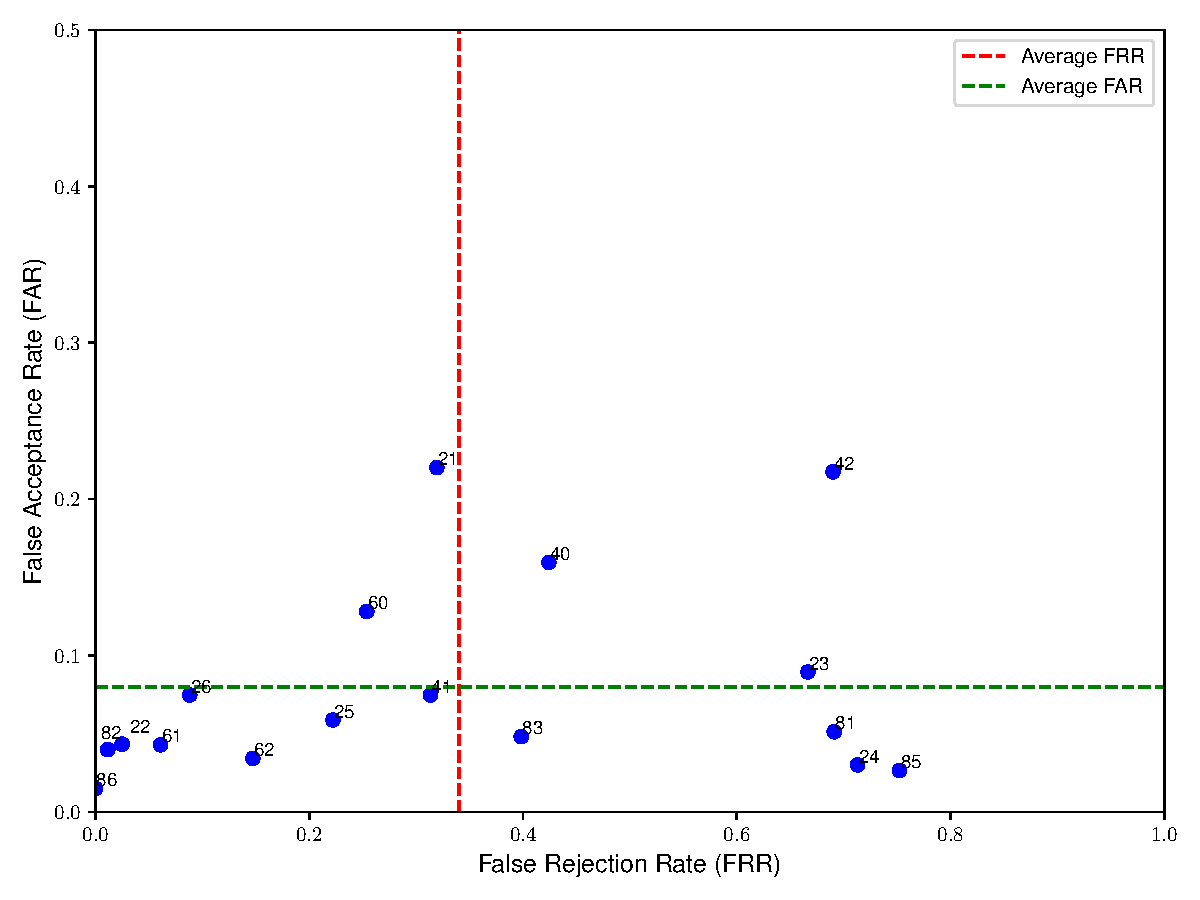
\includegraphics[width=\textwidth]{images/far_vs_frr.pdf} 	
	\caption{False acceptance rate vs False rejection rate.}
	\label{fig:frr_vs_far_all_models_base}
\end{figure}

Figure \ref{fig:frr_vs_far_all_models_base} demonstrates the large discrepancy between the models. At the same threshold level of some models were able to achieve a FAR and FRR score of below 10\%, while other failed to recognize over half of examples in the positive class. \\
This first group comprises of models for users 86, 62, 82, 25, 26 and 61. These models were able to learn and generalize well to the test dataset.
The other major group of models were those with an unacceptably high FAR of over 45\% and a below average FAR score. These would include models for users 81, 24, 60, 40 and 23. The reason for such high FAR could be twofold, either the models simply failed to generalize to unseen positive example, or they did, but at a lower confidence level than the established threshold. Other models have varying performance and are hard to categorize into coherent groups.

\subsection{Equal Error Rate} \label{subsec_eer}
To calculate the equal error rate, the decision threshold needs to be adjusted, which can be done globally, for all models or at a per--model level. We chose to report both ways to calculate this metric. 

The global EER was calculated to illustrate the performance of the whole collection using one value.
\begin{itemize}
	\item[] Equal Error Rate: 0.157
	\item[] Threshold: 0.20
\end{itemize}
A low value of the decision threshold was necessary to achieve an equal error rate. This suggest that most of the models are unable to recognize positive examples with a high degree on confidence. Such a low value would not make sense in an applied setting and in the context of system developed in this project. 

The per model EER can be used to examine the differences between the models.\\
Is is calculated by finding equal error rate decision threshold for each model separately.
The results are shown in table \ref{table:EER_separate}.
\begin{center}
	\begin{table}[H]
		\begin{center}
			\begin{tabular}{ |c|c|c| } 
				\hline
				User ID & Equal Error Rate & Decision threshold \\
				\hline
				\hline
				21 & 0.124 & 0.95 \\
				\hline
				22 & 0.026 & 0.95 \\
				\hline
				23 & 0.245 & 0.40 \\
				\hline
				24 & 0.270 & 0.05 \\
				\hline
				25 & 0.037 & 0.85 \\
				\hline
				26 & 0.059 & 0.80 \\
				\hline
				40 & 0.200 & 0.05 \\
				\hline
				41 & 0.081 & 0.35 \\
				\hline
				42 & 0.163 & 0.45 \\
				\hline
				60 & 0.176 & 0.05 \\
				\hline
				61 & 0.066 & 0.80 \\
				\hline
				62 & 0.038 & 0.85 \\
				\hline
				81 & 0.392 & 0.05 \\
				\hline
				82 & 0.026 & 0.95 \\
				\hline
				83 & 0.220 & 0.05 \\
				\hline
				85 & 0.131 & 0.75 \\
				\hline
				86 & 0.028 & 0.90 \\
				\hline
				\hline
				Average & 0.133 & -- \\
				\hline
			\end{tabular}
		\end{center}
		\caption{Per model equal error rate.}
		\label{table:EER_separate}
	\end{table}
\end{center}

Table \ref{table:EER_separate} illustrates the difference in the ability of the models to generalize to unseen positive examples. This can be seen further by examining the change of FAR and FRR score with respect to the decision threshold, which is show in figure \ref{fig:far_ffr_all_thresholds}. 

\begin{figure}[H]
	\centering
	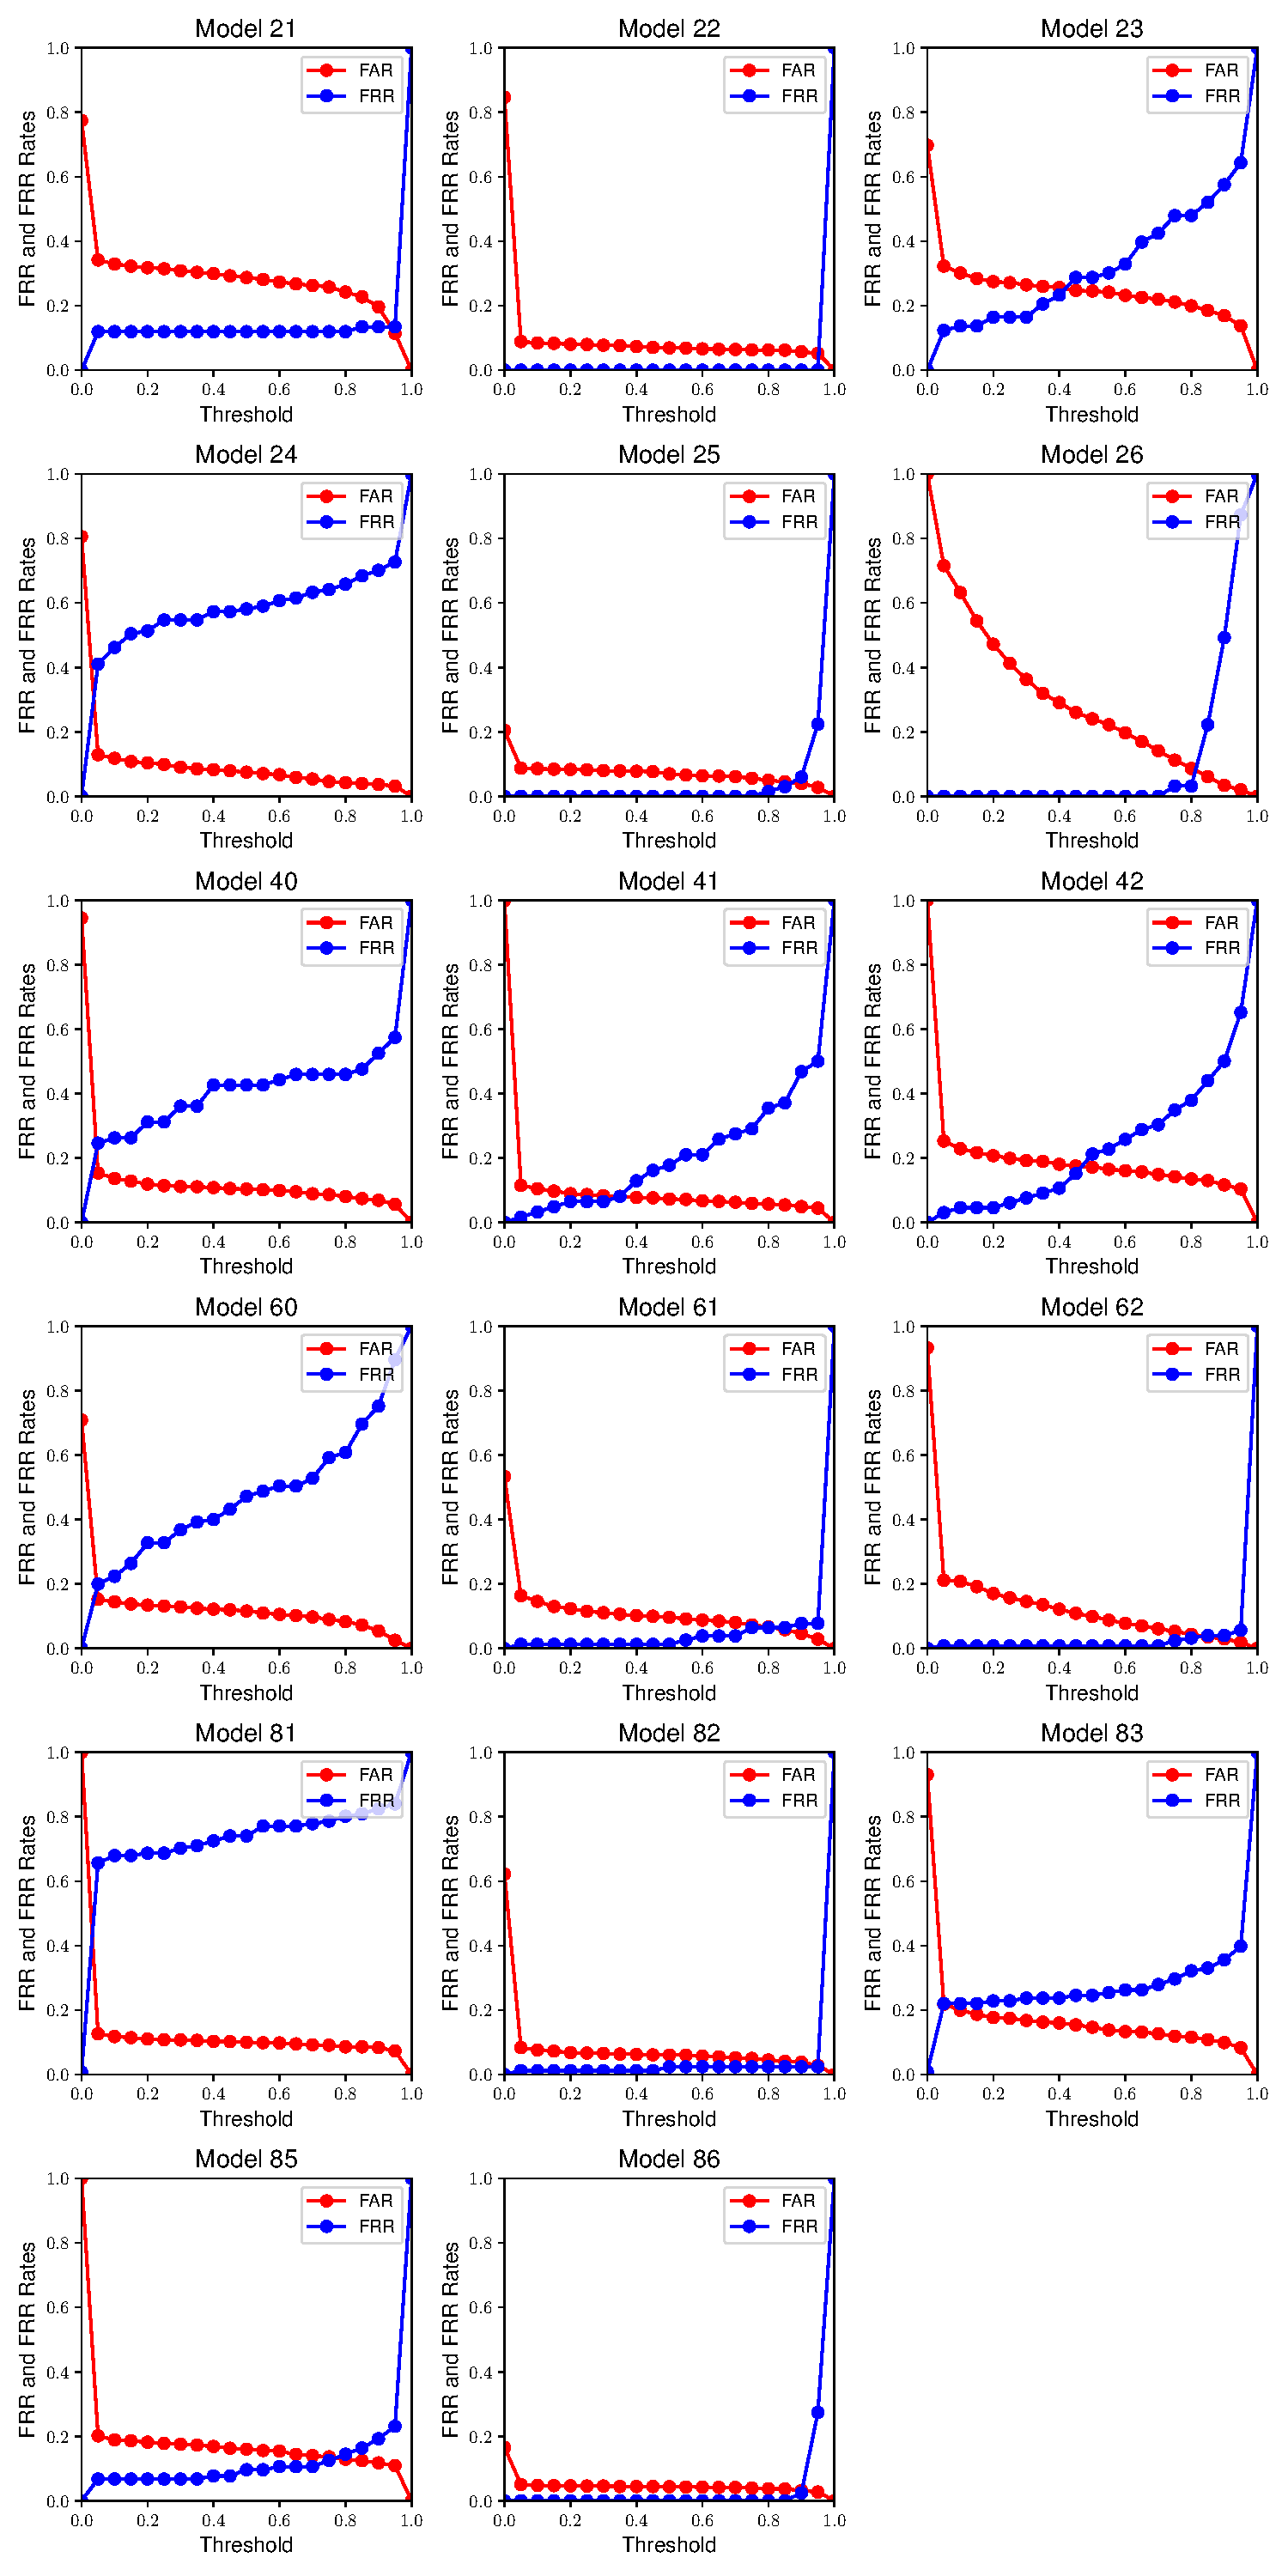
\includegraphics[width=.8\textwidth]{images/far_frr_curves_all_models_subplots.pdf} % Replace 'example.pdf' with your PDF file name
	\caption{Change of FAR and FRR score with respect to decision threshold.}
	\label{fig:far_ffr_all_thresholds}
\end{figure}

These plots shows the relationship between FAR, FRR and the decision threshold in more detail. The point at which the two lines cross is the EER. Worth noting is the large variation in the threshold at which EER is achieved. Models for users 21, 22, 25, 26, 61, 62, 82, 85, and 86 reach an equal error rate at or above a threshold of 0.8, which indicates a high degree of confidence in the prediction of the positive class. These models have a lower EER than models with lower threshold values. To ilustrate this , table \ref{EER_separate} sorted by EER is given below.

\begin{center}
	\begin{table}[H]
		\begin{center}
			\begin{tabular}{ |c|c|c| } 
				\hline
				User ID & Equal Error Rate & Decision threshold \\
				\hline
				\hline
				22 & 0.026 & 0.95 \\
				\hline
				82 & 0.026 & 0.95 \\
				\hline
				86 & 0.028 & 0.9 \\
				\hline
				25 & 0.037 & 0.85 \\
				\hline
				62 & 0.038 & 0.85 \\
				\hline
				26 & 0.059 & 0.8 \\
				\hline
				61 & 0.066 & 0.8 \\
				\hline
				41 & 0.081 & 0.35 \\
				\hline
				21 & 0.124 & 0.95 \\
				\hline
				85 & 0.131 & 0.75 \\
				\hline
				42 & 0.163 & 0.45 \\
				\hline
				60 & 0.176 & 0.05 \\
				\hline
				40 & 0.2 & 0.05 \\
				\hline
				83 & 0.22 & 0.05 \\
				\hline
				23 & 0.245 & 0.4 \\
				\hline
				24 & 0.27 & 0.05 \\
				\hline
				81 & 0.392 & 0.05 \\
				\hline
			\end{tabular}
		\end{center}
		\caption{Sorted per model equal error rate.}
		\label{table:EER_separate_sorted}
	\end{table}
\end{center}

A outlier in this trend is model 41, which achieves an equal error rate of 8.1\% at a 0.35 decision threshold, outperforming models with much higher decision thresholds. Outliers like this suggest, that a better approach than choosing one decision threshold could be to determine them on a per model basis. Such threshold could be chosen once, on some portion of the user training data through cross--validation, although such approach would lengthen the training process. Alternatively such value could be adjusted dynamically, based on how often a user fails to be authenticated using the model. Such considerations could be an area of further research as they fall outside the scope of this project.\\
Additionally, because a global decision forces poor performance on otherwise well performing models, we believe that the average per model EER is a better metric to use than the global EER and will as such it will be used in the rest of this chapter.\\
Another interesting examples is that of model 21, for which the FRR is almost constant, at a value of around 12\%. This indicates that all examples are recognized with a high degree of confidence, except those 12\%, which could indicate that the user changes writing styles for part of the final input or that the training data failed to capture some characteristic of the writing style.

\subsection{Confusion matrix for all users}
To evaluate the each model's performance, every model was tested on the input of every user. The results of this test are shown in figure \ref{fig:all_models_5_len40}. The values in this matrix represent the percentage of examples classified as positive. It is important to note that the values in this matrix have a different interpretation depending on their position. The values on the diagonal represent the percentage of correctly classified positive example (True Positives) -- the recall of the model. For an ideal classifier these values would equal 100. The values outside the diagonal represent the percentage of incorrectly classified negative examples (False Positives). For an ideal classifier these values would equal 0.

\begin{figure}[H]
	\centering
	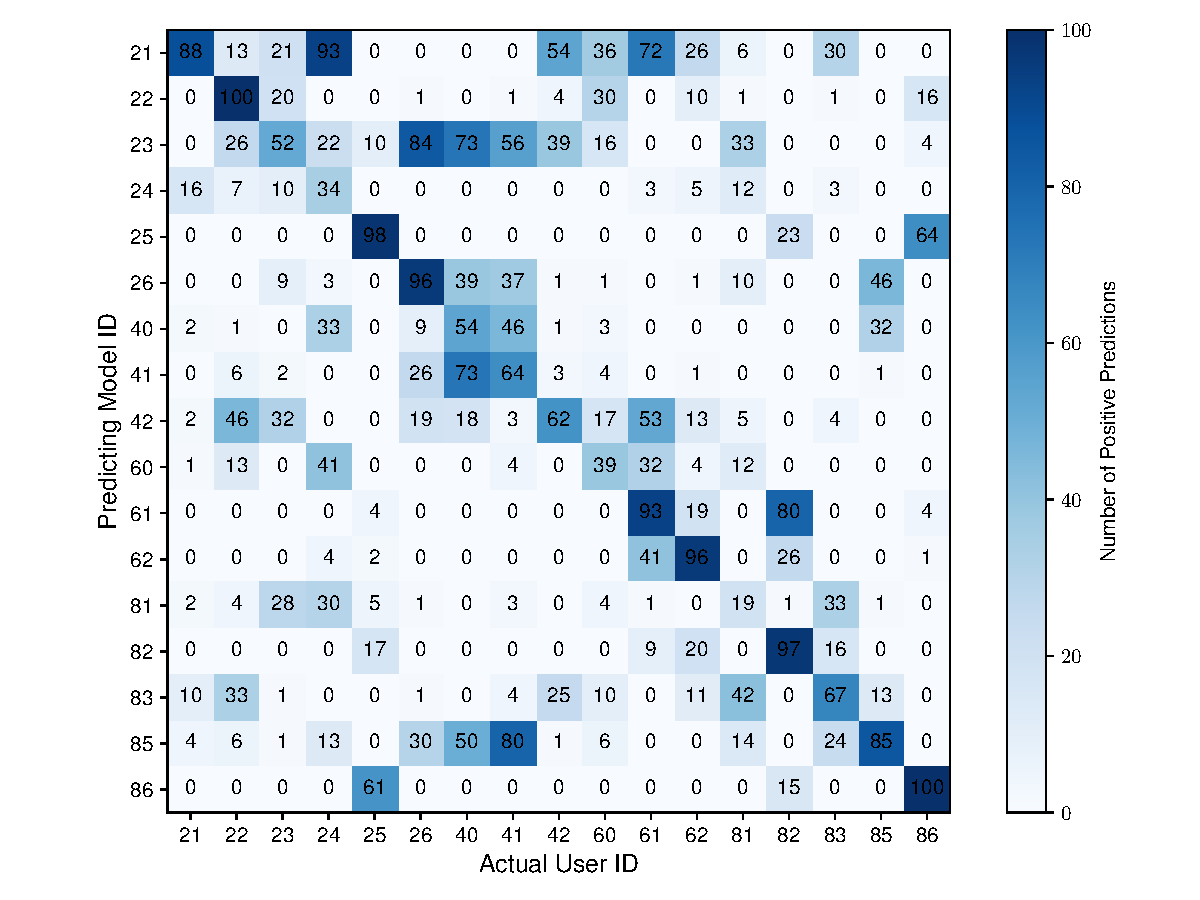
\includegraphics[width=\textwidth]{images/all_models_5_len40.pdf} % Replace 'example.pdf' with your PDF file name
	\caption{Matrix showing the percentage of examples classified as positive for all model--user pairs.}
	\label{fig:all_models_5_len40}
\end{figure}

Figure \ref{fig:all_models_5_len40} demonstrates the different errors made by individual models. More precisely, it shows which users share a similarity and therefore cause confusion for the models. For example models for users 25 and 86 perform very well for all inputs except each other. However this is not true for all models, as the model for user 61 makes mistakes when classifying the input for user 82. The inverse is not true, the model for user 82 does not misclassify user 61 data at a higher rate than others.

\section{Input features}
This section will compare the impact of input encodings on the final model performance, as measured by the average FAR and FRR, as well as the average per model EER value. The impact of these changes were measured by changing only one hyperparameters, while all others remain the same as shown in table \ref{table:hyperparams}. The results shown below compare performance on the testing dataset, so that these values can be contrasted with what was discussed in the previous section. As was mentioned previously, this is not how these features were selected.

\subsection{Input sequence length}
The theoretical impact of input length, discussed in the section on graph creation, would suggest that there exists an optimal sequence length. Making the sequence shorter would result in graphs that do not have enough structure, for example a chain of nodes, or edge data to make the correct prediction possible. Make the sequence longer would result in graph that is too dense or cause the averages calculated per node to become too aggregated.\\


\begin{center}
	\begin{table}[H]
		\begin{center}
			\begin{tabular}{ |c|c|c|c| } 
				\hline
				Input sequence length & FAR & FRR & EER \\
				\hline
				30 & 0.101 & 0.332 & 0.180 \\
				\hline
				40 & 0.092 & 0.264 & 0.133 \\
				\hline
				50 & 0.098 & 0.232 & 0.135 \\
				\hline
				60 & 0.079 & 0.307 & 0.158 \\
				\hline
				70 & 0.083 & 0.391 & 0.176 \\
				\hline
			\end{tabular}
		\end{center}
		\caption{Comparison of performance with different lengths of input sequence.}
		\label{table:len_vs_perf}
	\end{table}
\end{center}


Table \ref{table:len_vs_perf} does partly support the theoretical expectation, as models trained on input sequences of length 30, 60 and 70 achieve much higher EER scores than those trained with lengths of 40 and 50. There is a very small difference in the way these collections of models perform on these aggregated metrics. 
With the difference in the EER scores being this low, it is unclear which collection of models performed better on testing dataset.
However, interesting differences appear when comparing on a per model basis, as the changes in models were not uniform. The impact of 3 selected models is shown in figure \ref{fig:selected_frr_vs_far}. 

\begin{figure}[H]
	\centering
	\subfloat[Plots for input of length 40]{
		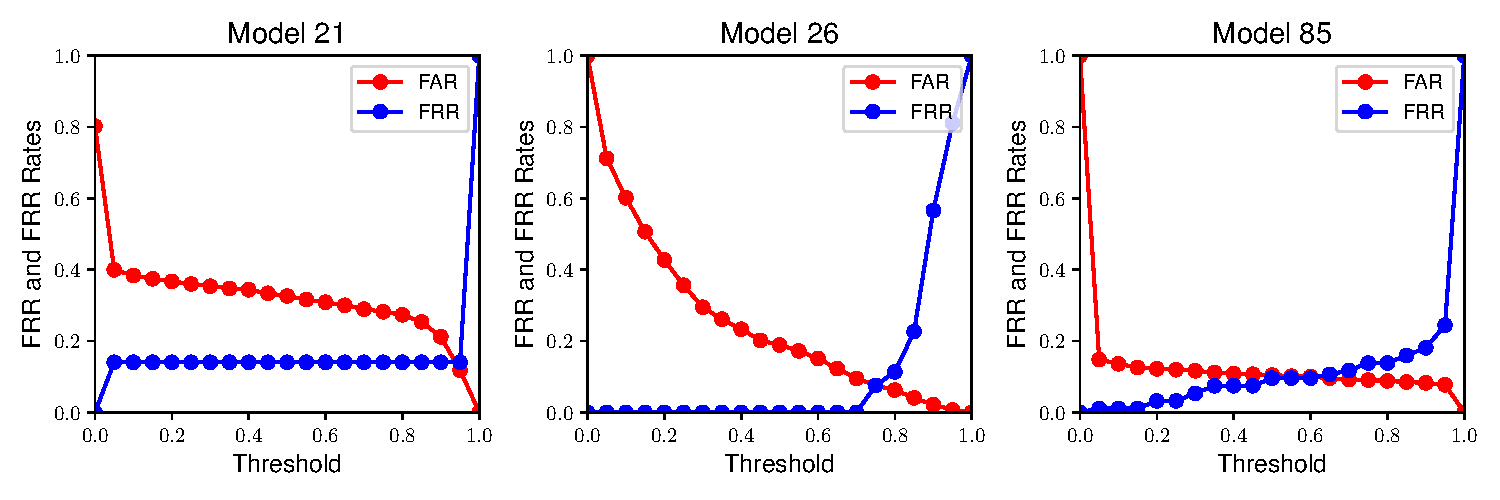
\includegraphics[width=\textwidth]{images/selected_far_vs_frr_len40.pdf}
	}

	\subfloat[Plots for input of length 50]{
		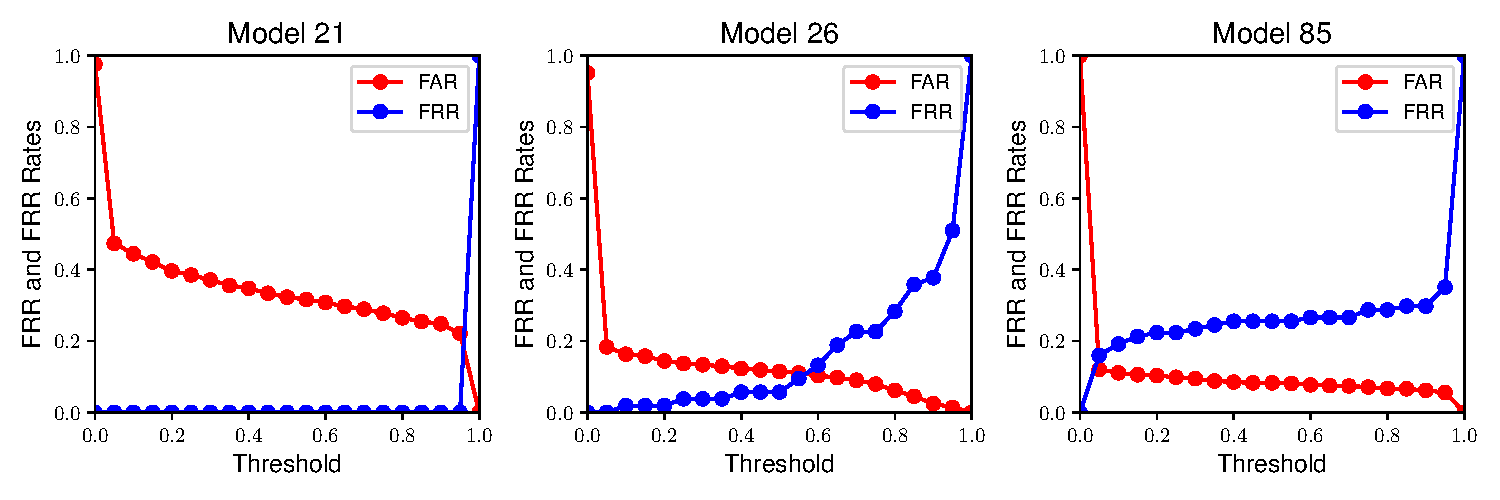
\includegraphics[width=\textwidth]{images/selected_far_vs_frr_len50.pdf}
	}
	\caption{Comparison of selected FAR and FRR plots for different input lengths}%
	\label{fig:selected_frr_vs_far}%
\end{figure}

The model for user 21 shows a clear improvement as the unrecognized examples discussed in subsection \ref{subsec_eer} are now correctly classified. Conversely, the model for user 26 now classifies its positive examples with less confidence and showed an increase for an EER of 5.9\% to 10.2\%. For model 85 the change in length did not impact the EER, however it moved the decision threshold significantly.\\
What these comparison demonstrate is that it is hard to reason about model performance across different input sequence lengths and small change has a large impact even on a per model bases.

\subsection{Character encoding}
The results of comparing methods of character information in nodes are shown in table
\ref{table:char_encoding}.

\begin{center}
	\begin{table}[H]
		\begin{center}
			\begin{tabular}{ |c|c|c|c| } 
				\hline
				Character encoding method & FAR & FRR & EER \\
				\hline
				\textit{Normalized Base Letter Encoding} & 0.092 & 0.264 & 0.133 \\
				\hline
				\textit{Compact Alphabet Encoding} & 0.082 & 0.339 & 0.161 \\
				\hline
				\textit{Full One-Hot Encoding} & 0.070 & 0.397 & 0.197 \\
				\hline
			\end{tabular}
		\end{center}
		\caption{Comparison of performance with different edge data encoding methods.}
		\label{table:char_encoding}
	\end{table}
\end{center}

Table \ref{table:char_encoding} shows the more aggregating methods outperform those with less compact. The lower FAR might suggest that these models try to capture more complex features and thus overfit the data.

\subsection{Edge data encoding}

\begin{center}
	\begin{table}[H]
		\begin{center}
			\begin{tabular}{ |c|c|c|c| } 
				\hline
				Edge encoding method & FAR & FRR & EER \\
				\hline
				\textit{Two dimensional vector of values per node} & 0.069 & 0.666 & 0.395 \\
				\hline
				\textit{Two values per node} & 0.092 & 0.264 & 0.133 \\
				\hline
			\end{tabular}
		\end{center}
		\caption{Comparison of performance with different edge data encoding methods.}
		\label{table:egde_encoding_comp}
	\end{table}
\end{center}

Table \ref{table:egde_encoding_comp} shows the superiority of the \textit{Two values per node} encoding method. While the average far remains comparable, FRR, and thus the EER, differ by a large amount. This might be cause by the same reasons as the difference between character encoding methods. The method with less aggregation performs worse, as the model might not have seen all possible two letter combinations and failed to generalize.


\subsection{Accelerometer Data}
As was mentioned in subsection \ref{accel_subsection}, accelerometer data was collected alongside keystroke information. While the use of accelerometer data lead to modes that quickly achieved low loss on the training data, these results did not generalize to validation and test data. An example of an increase in generalization error for user \myworries{TODOO} is shown below.

\section{Class imbalance}
Another point of experimentation was class balance in the training data. The baseline model was trained on a dataset with two times more positive examples than negative examples. A bigger proportion of positive examples was chosen experimentally, as it resulted in models that perform better at recognizing the positive class. \\ 
The negative examples were sampled uniformly from all other users, with an offset such that the negative examples for some user were taken from the whole input text. This works for the number of users in the dataset. However, as the number of users grows, and the length of input sequence stays fixed, at some point each model needs to be trained only on a subset of the negative class input texts. At that point some models could fail to generalize to unseen negative examples. 
While solving such problem lies outside the scope of this project, the impact of using more negative examples in the training process was measured and the results are presented in table \ref{table:egde_encoding_comp}.


\begin{center}
	\begin{table}[H]
		\begin{center}
			\begin{tabular}{ |c|c|c|c| } 
				\hline
				Positive to Negative Ratio & FAR & FRR & EER \\
				\hline
				\textit{2:1} & 0.092 & 0.264 & 0.133 \\
				\hline
				\textit{1:1} & 0.080 & 0.340 & 0.177 \\
				\hline
				\textit{1:2} & 0.033 & 0.506 & 0.220 \\
				\hline
			\end{tabular}
		\end{center}
		\caption{Impact of positive to negative ratio on model collection performance.}
		\label{table:egde_encoding_comp}
	\end{table}
\end{center}

At higher percentage of negative examples were classified correctly, as indicated by the lower FAR, this comes at the expense of a large drop in the FRR score, to almost half of positive examples being dropped in the case of \textit{1:2} class balance. This means that the collection of models generalized poorly to unseen positive examples, to a degree that would be unacceptable. This can also be seen when comparing the average recall scores across these two collections of models, which dropped from \textit{0.7357} to \textit{0.692} and \textit{0.494} when the number of negative examples were doubled. 
